\documentclass{article}

\usepackage{postprocess/context/arxiv}

\usepackage[utf8]{inputenc} % allow utf-8 input
\usepackage{amsmath}
\usepackage[T1]{fontenc}    % use 8-bit T1 fonts
\usepackage{hyperref}       % hyperlinks
\usepackage{url}            % simple URL typesetting
\usepackage{booktabs}       % professional-quality tables
\usepackage{amsfonts}       % blackboard math symbols
\usepackage{nicefrac}       % compact symbols for 1/2, etc.
\usepackage{microtype}      % microtypography
\usepackage{graphicx}
\usepackage{natbib}
\usepackage{doi}
\usepackage{float}
\usepackage{subcaption}
\usepackage{wrapfig}

\title{Causal Discovery Report on Abalone}

\author{ \href{https://orcid.org/0000-0000-0000-0000}{
\includegraphics[scale=0.06]{postprocess/context/orcid.pdf}\hspace{1mm}Causal Copilot}}

\renewcommand{\headeright}{Technical Report}
\renewcommand{\undertitle}{Technical Report}

\hypersetup{
pdftitle={Causal Discovery Report on Abalone},
pdfauthor={Causal Copilot},
pdfkeywords={Causal Discovery, Large Language Model, PC, Abalone},
}

\begin{document}
\maketitle

\begin{abstract}
This report presents a causal discovery analysis of a dataset consisting of various measurements related to abalones, including age, length, shell weight, diameter, height, whole weight, shucked weight, and viscera weight. We employed a comprehensive methodology utilizing three algorithms—PC, GES, and NOTEARS—selected based on data characteristics and suitability for continuous variables. A detailed graph tuning process was conducted, integrating Bootstrap confidence intervals and suggestions from a large language model to refine the causal graph. Our analysis revealed significant causal relationships, such as the influence of age on diameter and viscera weight, and the interconnections between various weight metrics. While our findings indicate robust relationships supported by expert knowledge, some edges exhibit low confidence, indicating a need for further investigation. This work contributes to a better understanding of the growth dynamics of abalones, enhancing insights into their biological and commercial significance.
\end{abstract}

\keywords{Causal Discovery, Large Language Model, PC, Abalone}

\raggedbottom
\section{Introduction}
In this report, we will conduct a causal discovery analysis on a dataset comprising various measurements of abalones, a type of marine mollusk. The dataset includes multiple variables such as age, length, shell weight, diameter, height, whole weight, shucked weight, and viscera weight. Each of these variables offers valuable insights into the growth patterns, health status, and reproductive maturity of abalones. Understanding the potential causal relationships among these variables is crucial, as it can elucidate how factors like age influence physical dimensions and, in turn, impact weight measurements crucial for commercial fishing. By employing causal discovery techniques, we aim to reveal underlying patterns and dependencies within this biological context, while also considering external factors such as environmental conditions and reproductive cycles that may affect these dynamics.

\section{Background Knowledge}
\subsection{Detailed Explanation about the Variables}
\begin{itemize}
\item \textbf{Age}: This variable represents the age of the abalones, which is often estimated by the number of rings on their shells. The age can give insight into growth patterns and reproductive maturity.
\item \textbf{Length}: This variable indicates the length of the abalone measured from the anterior end to the posterior end of the shell. It is a common measure in marine biology to assess the size of the organism.
\item \textbf{Shell weight}: This is the weight of the abalone’s shell, usually measured in grams. The shell weight can provide information about the density and health of the abalone, as well as its growth stage.
\item \textbf{Diameter}: The diameter is the measurement across the shell at its widest point. This variable can be related to the overall growth and maturity of the abalone.
\item \textbf{Height}: This variable measures the height of the abalone's shell from the bottom to the top. Height, along with length and diameter, contributes to understanding the abalone's shape and size.
\item \textbf{Whole weight}: This is the total weight of the abalone, including its shell, flesh, and any other components. Whole weight can give a comprehensive view of the abalone's biomass and condition.
\item \textbf{Shucked weight}: This weight refers to the weight of the abalone's meat after the shell has been removed. This variable is crucial in commercial fishing and culinary contexts, where the meat is the primary product.
\item \textbf{Viscera weight}: This variable measures the weight of the internal organs of the abalone. Viscera weight can be important for understanding the overall health and condition of the organism, and it may be related to reproductive health.
\end{itemize}

\subsection{Possible Causal Relations among these Variables}

\begin{minipage}[t]{0.7\linewidth}
\begin{itemize}
\item \textbf{Age $\rightarrow$ Length}: The age of the abalone influences its length as older abalones tend to grow larger due to increased time for growth and development.

\item \textbf{Age $\rightarrow$ Diameter}: The age of the abalone affects its diameter, as older abalones generally exhibit a larger diameter as part of their growth process.

\item \textbf{Age $\rightarrow$ Height}: As abalones age, they typically grow taller, thus the age influences the height of the shell.

\item \textbf{Length $\rightarrow$ Whole weight}: An increase in length of the abalone is likely to contribute to an increase in the whole weight since larger abalones contain more mass.

\item \textbf{Diameter $\rightarrow$ Whole weight}: The diameter of the abalone is associated with its overall size, which will naturally lead to increased whole weight as it grows.

\item \textbf{Height $\rightarrow$ Whole weight}: An increase in the height of the abalone suggests a larger size and subsequently a higher whole weight.

\item \textbf{Whole weight $\rightarrow$ Shucked weight}: The whole weight of the abalone affects the shucked weight directly, as more overall mass corresponds to more available meat after the shell is removed.

\item \textbf{Whole weight $\rightarrow$ Viscera weight}: An increase in whole weight typically results in an increase in viscera weight, reflecting the overall health and organ size related to body mass.

\item \textbf{Shucked weight $\rightarrow$ Viscera weight}: The weight of the abalone's meat can influence the weight of the viscera, as healthier and larger abalones usually contain proportionally larger internal organs. 

\item \textbf{Shell weight $\rightarrow$ Age}: The weight of the shell may correlate to the age of the abalone, as older abalones tend to have heavier and more mature shells, reflecting their developmental history.
\end{itemize}
\end{minipage}
\hspace{0.05\textwidth}
\begin{minipage}[t]{0.3\linewidth}
\begin{figure}[H]
\centering
\resizebox{\linewidth}{!}{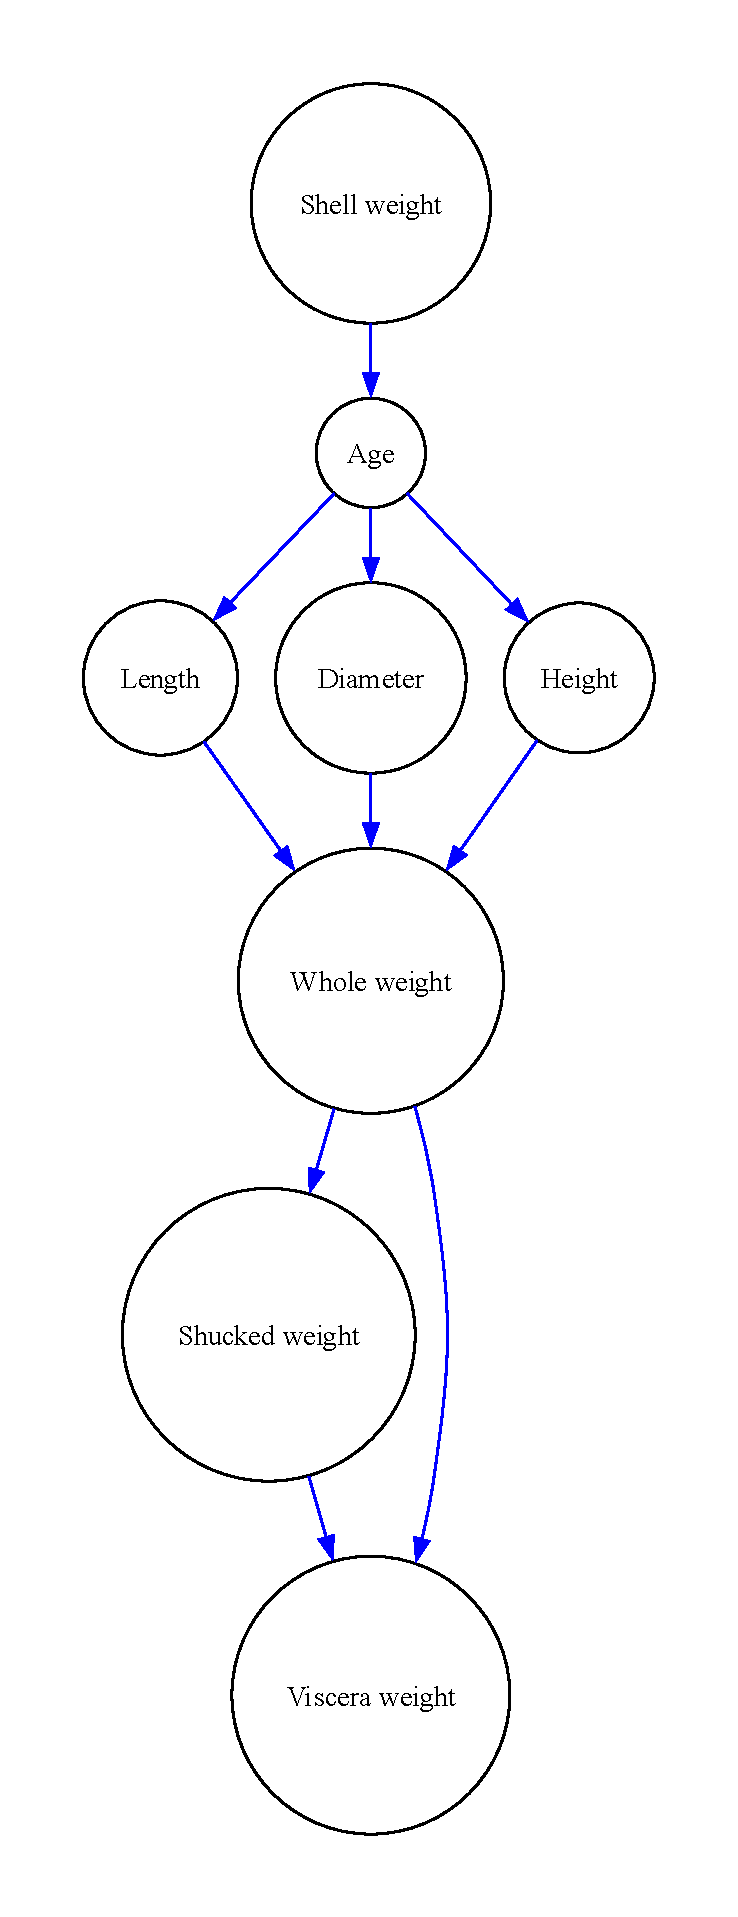
\includegraphics[height=0.3\textheight]{./demo_data/20241104_121546/Abalone/output_graph/potential_relation.pdf}}
\caption{\label{fig:relation}Possible Causal Relation Graph}
\end{figure}
\end{minipage}

\section{Dataset Descriptions and EDA}
The following is a preview of our original dataset.

\begin{table}[H]
    \centering
    \caption{Dataset Preview}
    \begin{tabular}{rrrrrrrr}
\toprule
 Age &  Length &  Shell weight &  Diameter &  Height &  Whole weight &  Shucked weight &  Viscera weight \\
\midrule
15.0 &   0.455 &         0.365 &     0.095 &  0.5140 &        0.2245 &          0.1010 &           0.150 \\
 7.0 &   0.350 &         0.265 &     0.090 &  0.2255 &        0.0995 &          0.0485 &           0.070 \\
 9.0 &   0.530 &         0.420 &     0.135 &  0.6770 &        0.2565 &          0.1415 &           0.210 \\
10.0 &   0.440 &         0.365 &     0.125 &  0.5160 &        0.2155 &          0.1140 &           0.155 \\
 7.0 &   0.330 &         0.255 &     0.080 &  0.2050 &        0.0895 &          0.0395 &           0.055 \\
\bottomrule
\end{tabular}
\end{table}

\subsection{Data Properties}
We employ several statistical methods to identify data properties.

The shape of the data, data types, and missing values are assessed directly from the dataframe.
Linearity is evaluated using Ramsey’s RESET test, followed by the Benjamini \& Yekutieli procedure for multiple test correction.
Gaussian noise is assessed through the Shapiro-Wilk test, also applying the Benjamini \& Yekutieli procedure for multiple test correction.
Time-Series and Heterogeneity are derived from user queries.

Properties of the dataset we analyzed are listed below.

\begin{table}[H]
    \centering
    \caption{Data Properties}
    \begin{tabular}{rrrrrrr}
\toprule
Shape ($n$ x $d$) & Data Type & Missing Value & Linearity & Gaussian Errors & Time-Series & Heterogeneity \\
\midrule
(4177, 8)   & Continuous & False & False & False & False & False \\
\bottomrule
\end{tabular}
\end{table}

\subsection{Distribution Analysis}
The following figure shows distributions of different variables. The orange dash line represents the mean, 
and the black line represents the median. Variables are categorized into three types according to their distribution characteristics.

\begin{figure}[H]
\centering
\includegraphics[width=\linewidth]{./demo_data/20241104_121546/Abalone/output_graph/eda_dist.jpg}
\caption{\label{fig:dist}Distribution Plots of Variables}
\end{figure}

\begin{itemize}
\item Slight left skew distributed variables: Length, Shell Weight, Diameter, Whole Weight
\item Slight right skew distributed variables: Age, Height, Shucked weight, Viscera weight
\item Symmetric distributed variables: None
\end{itemize}

\subsection{Correlation Analysis}

\begin{minipage}[t]{0.5\linewidth}
In this analysis, we will categorize the correlation statistics of features in the dataset into three distinct categories: Strong correlations, Moderate correlations, and Weak correlations.

\begin{itemize}
\item Strong Correlated Variables: Shell weight and Length, Shell weight and Viscera weight, Diameter and Length, Height and Length, Whole weight and Height, Shucked weight and Height, Shucked weight and Whole weight, Viscera weight and Height
\item Moderate Correlated Variables: Length and Age, Shell weight and Age, Diameter and Age, Height and Age, Whole weight and Diameter, Viscera weight and Diameter, Shucked weight and Diameter, Viscera weight and Whole weight
\item Weak Correlated Variables: Shucked weight and Age, None
\end{itemize}
\vfill
\end{minipage}
\hfill
\begin{minipage}[t]{0.5\linewidth}
\begin{figure}[H]
\centering
\vspace{-1.5cm}
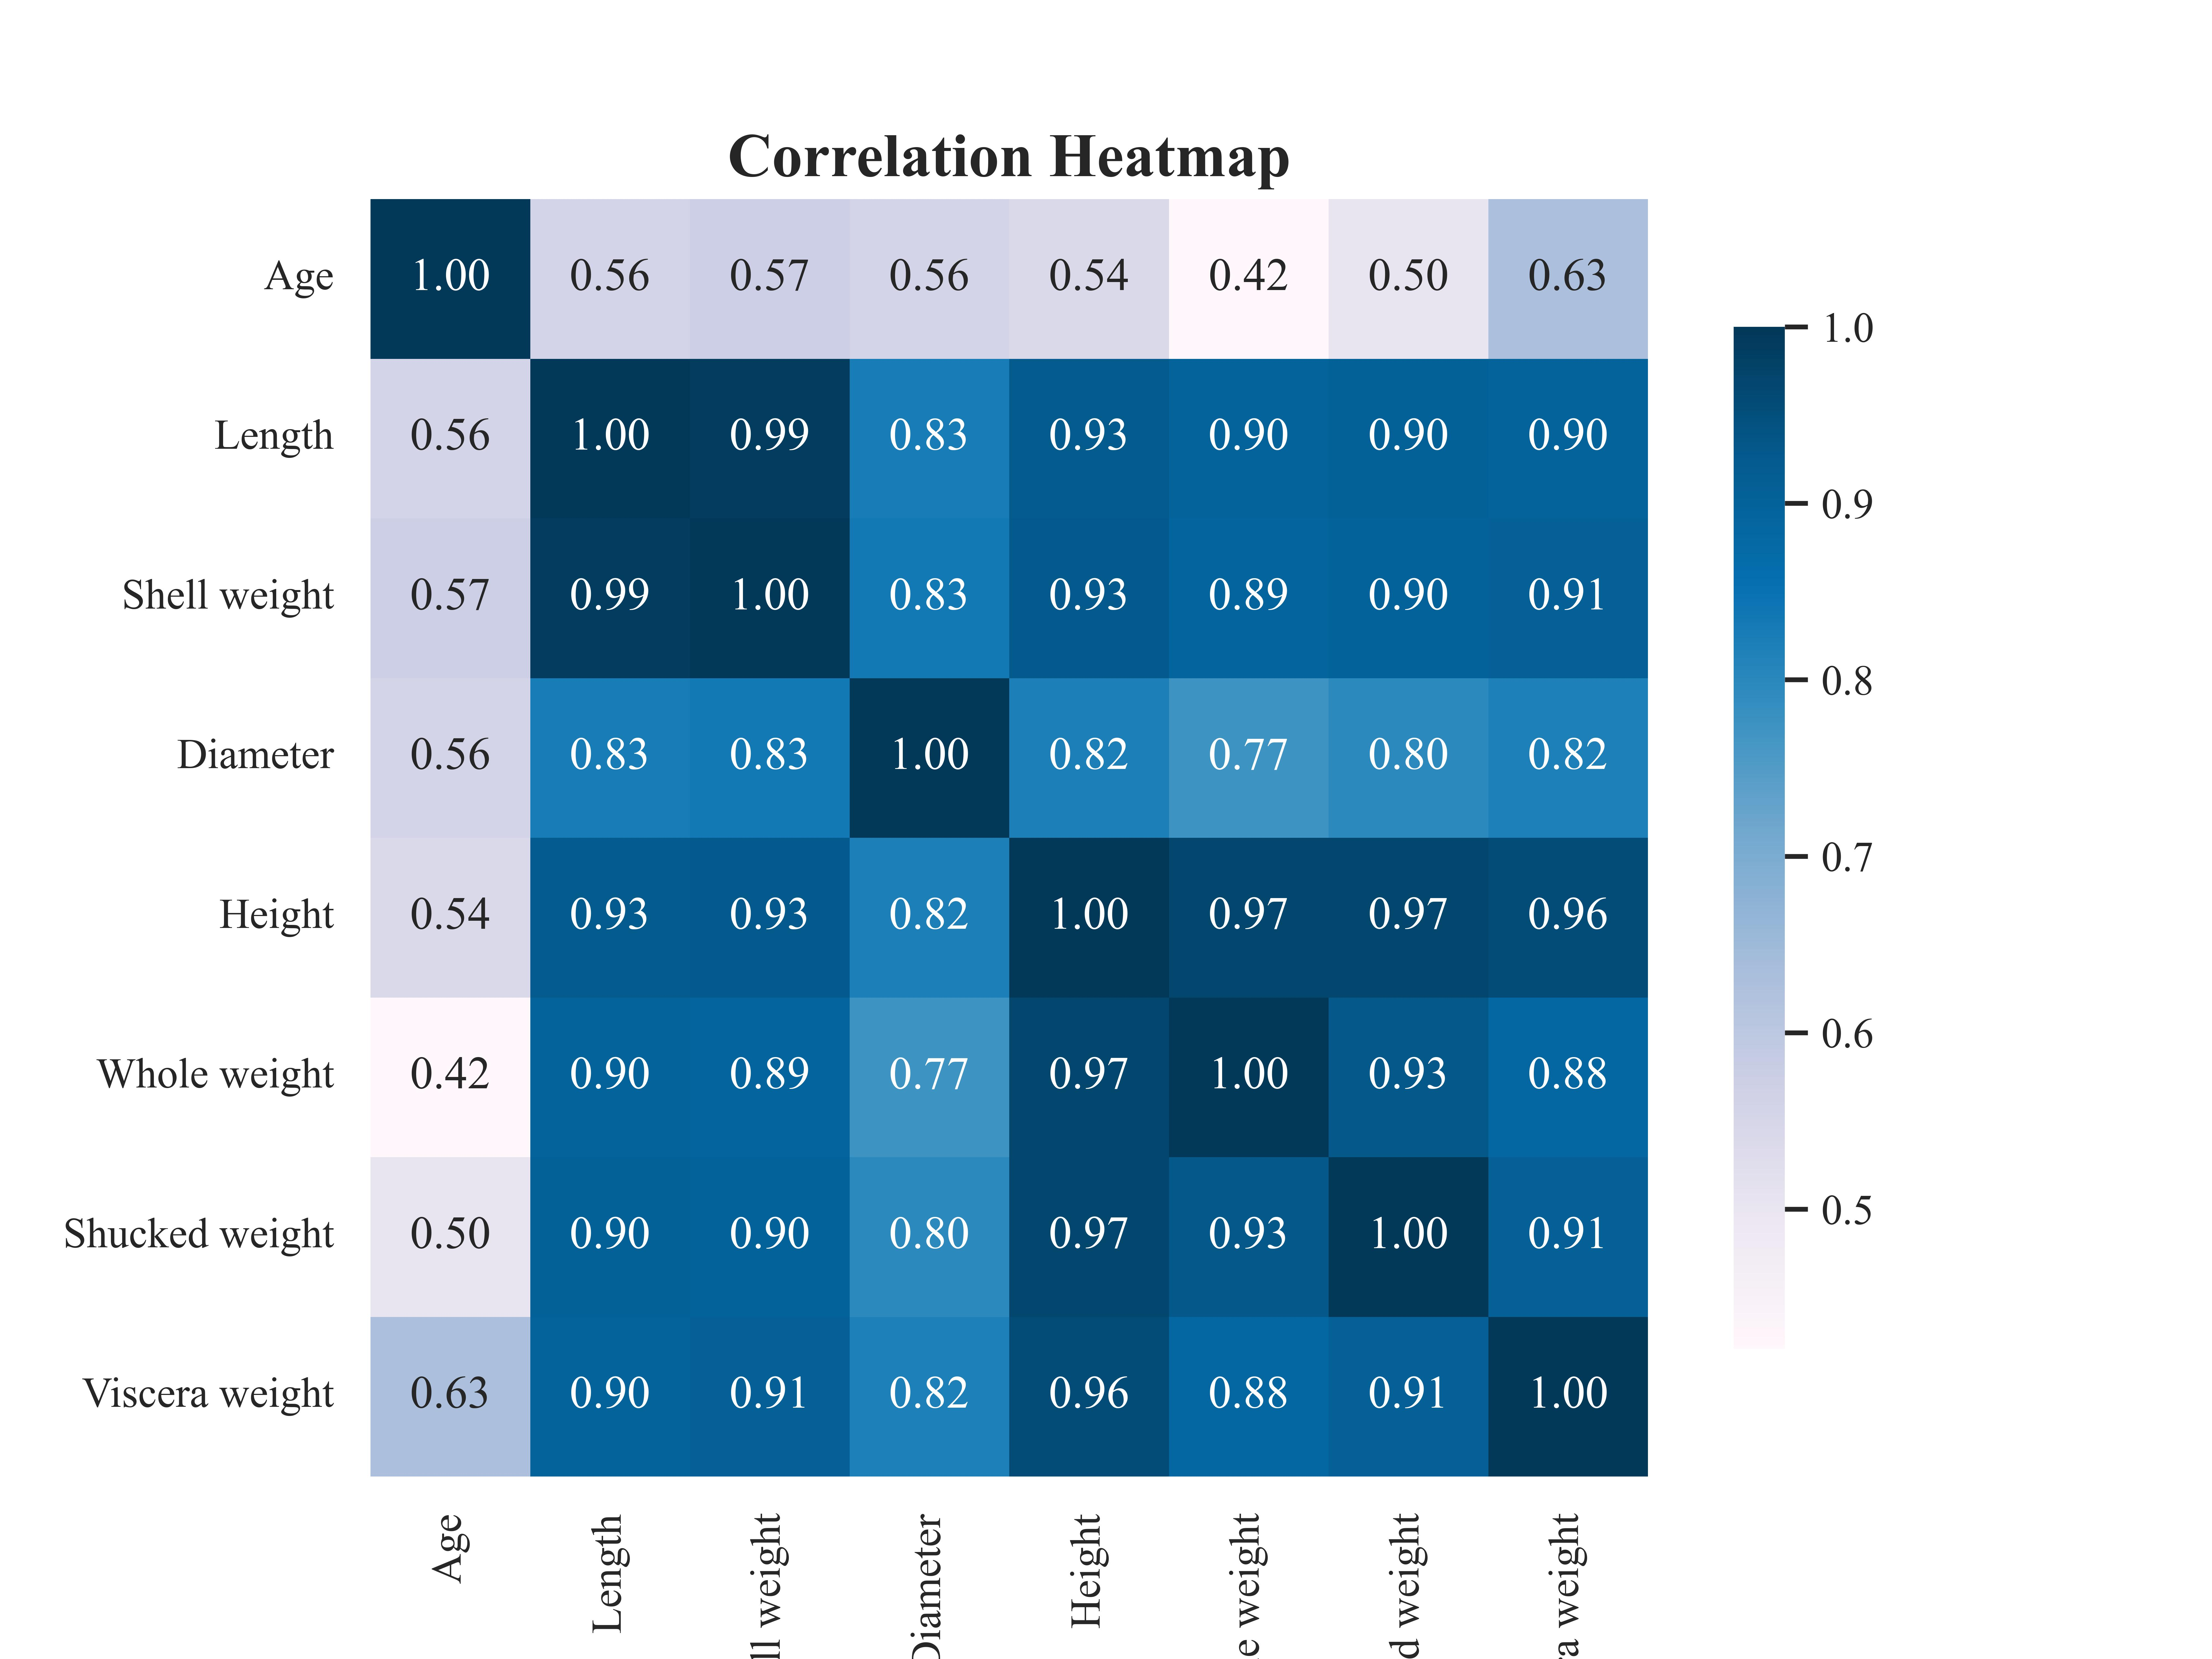
\includegraphics[width=\linewidth]{./demo_data/20241104_121546/Abalone/output_graph/eda_corr.jpg}
\caption{\label{fig:corr}Correlation Heatmap of Variables}
\end{figure}
\end{minipage}

\section{Discovery Procedure}

In this section, we provide a detailed description of the causal discovery process implemented by Causal Copilot. 
We also provide the chosen algorithms and hyperparameters, along with the justifications for these selections.

\subsection{Data Preprocessing}
In this initial step, we preprocessed the data and examined its statistical characteristics. 
This involved cleaning the data, handling missing values, and performing exploratory data analysis to understand distributions and relationships between variables.
                
\subsection{Algorithm Selection assisted with LLM}
Following data preprocessing, we employed a large language model (LLM) to assist in 
selecting appropriate algorithms for causal discovery based on the statistical characteristics of the dataset and relevant background knowledge. 
The top three chosen algorithms, listed in order of suitability, are as follows:   
        
\begin{itemize}
\item \textbf{PC}:
    \begin{itemize}
        \item \textbf{Description}: The PC algorithm is a constraint-based method that learns the structure of a causal graph from data by testing conditional independencies between variables. It constructs a directed acyclic graph (DAG) representing the causal relationships.
        \item \textbf{Justification}: Given the large sample size of 4177 and the absence of missing values, the PC algorithm is efficient for causal discovery. It balances computational efficiency with accuracy in identifying causal relationships, making it highly suitable for this dataset with continuous data types.
    \end{itemize}
                         
\item \textbf{GES}:
    \begin{itemize}
        \item \textbf{Description}: Greedy Equivalence Search (GES) is a score-based causal discovery algorithm that identifies the optimal causal structure by navigating the space of equivalence classes of Directed Acyclic Graphs (DAGs), optimizing through a scoring criterion.
        \item \textbf{Justification}: Considering the high dimensionality and continuous nature of the data without predominant linear relationships, GES can efficiently explore causal structures. Its ability to handle both Gaussian and non-Gaussian noise with flexibility in score functions makes it a suitable option given the dataset properties.
    \end{itemize}
                         
\item \textbf{NOTEARS}:
    \begin{itemize}
        \item \textbf{Description}: NOTEARS transforms the combinatorial problem of learning Directed Acyclic Graphs (DAGs) into a continuous optimization problem, suitable for large datasets and high-dimensional situations.
        \item \textbf{Justification}: NOTEARS is particularly suitable for this dataset due to its large size and continuous variables. The algorithm's ability to accommodate nonlinear relationships while being efficient makes it an excellent choice for discovering causal structures in datasets where traditional combinatorial methods may struggle.
    \end{itemize}
\end{itemize}
                    
\subsection{Hyperparameter Values Proposal assisted with LLM}
Once the algorithms were selected, the LLM aided in proposing hyperparameters 
for the chosen algorithm, which are specified below:
        
\begin{itemize}
\item \textbf{alpha}:
    \begin{itemize}
        \item \textbf{Value}: 0.05
        \item \textbf{Explanation}: Given the sample size of 4177, which falls within the range of 500-10000, an alpha value of 0.05 is appropriate. This balances the risk of false positives while maintaining sufficient sensitivity for the given sample size.
    \end{itemize}
                         
\item \textbf{indep\_test}:
    \begin{itemize}
        \item \textbf{Value}: fisherz
        \item \textbf{Explanation}: Since all variables in this dataset are continuous, Fisher's Z is the suitable choice for independence testing. It allows for well-established statistical methods tailored for continuous data, even though we need to be cautious due to the dataset's non-Gaussian errors.
    \end{itemize}
                         
\item \textbf{depth}:
    \begin{itemize}
        \item \textbf{Value}: -1
        \item \textbf{Explanation}: Using -1 allows for unlimited search depth, which is beneficial given the relatively large size of the dataset and the potential complexity of the relationships between the variables. This ensures thoroughness in causal discovery, although it might slightly impact computational efficiency.
    \end{itemize}     
\end{itemize}        

\subsection{Graph Tuning with Bootstrap and LLM Suggestion}
In the final step, we performed graph tuning with suggestions provided by the Bootstrap and LLM.
            
Firstly, we use the Bootstrap technique to get how much confidence we have on each edge in the initial graph.
If the confidence probability of a certain edge is greater than 95\% and it is not in the initial graph, we force it.
Otherwise, if the confidence probability is smaller than 5\% and it exists in the initial graph, we change it to the edge type with the highest probability.
            
After that, we utilize LLM to help us prune edges and determine the direction of undirected edges according to its knowledge repository.
In this step LLM can use background knowledge to add some edges that are neglected by Statistical Methods.
Voting techniques are used to enhance the robustness of results given by LLM, and the results given by LLM should not change results given by Bootstrap.

By integrating insights from both of Bootstrap and LLM to refine the causal graph, we can achieve improvements in graph's accuracy and robustness.
            
\section{Results Summary}

\subsection{Initial Graph}

\begin{figure}[H]
    \centering
    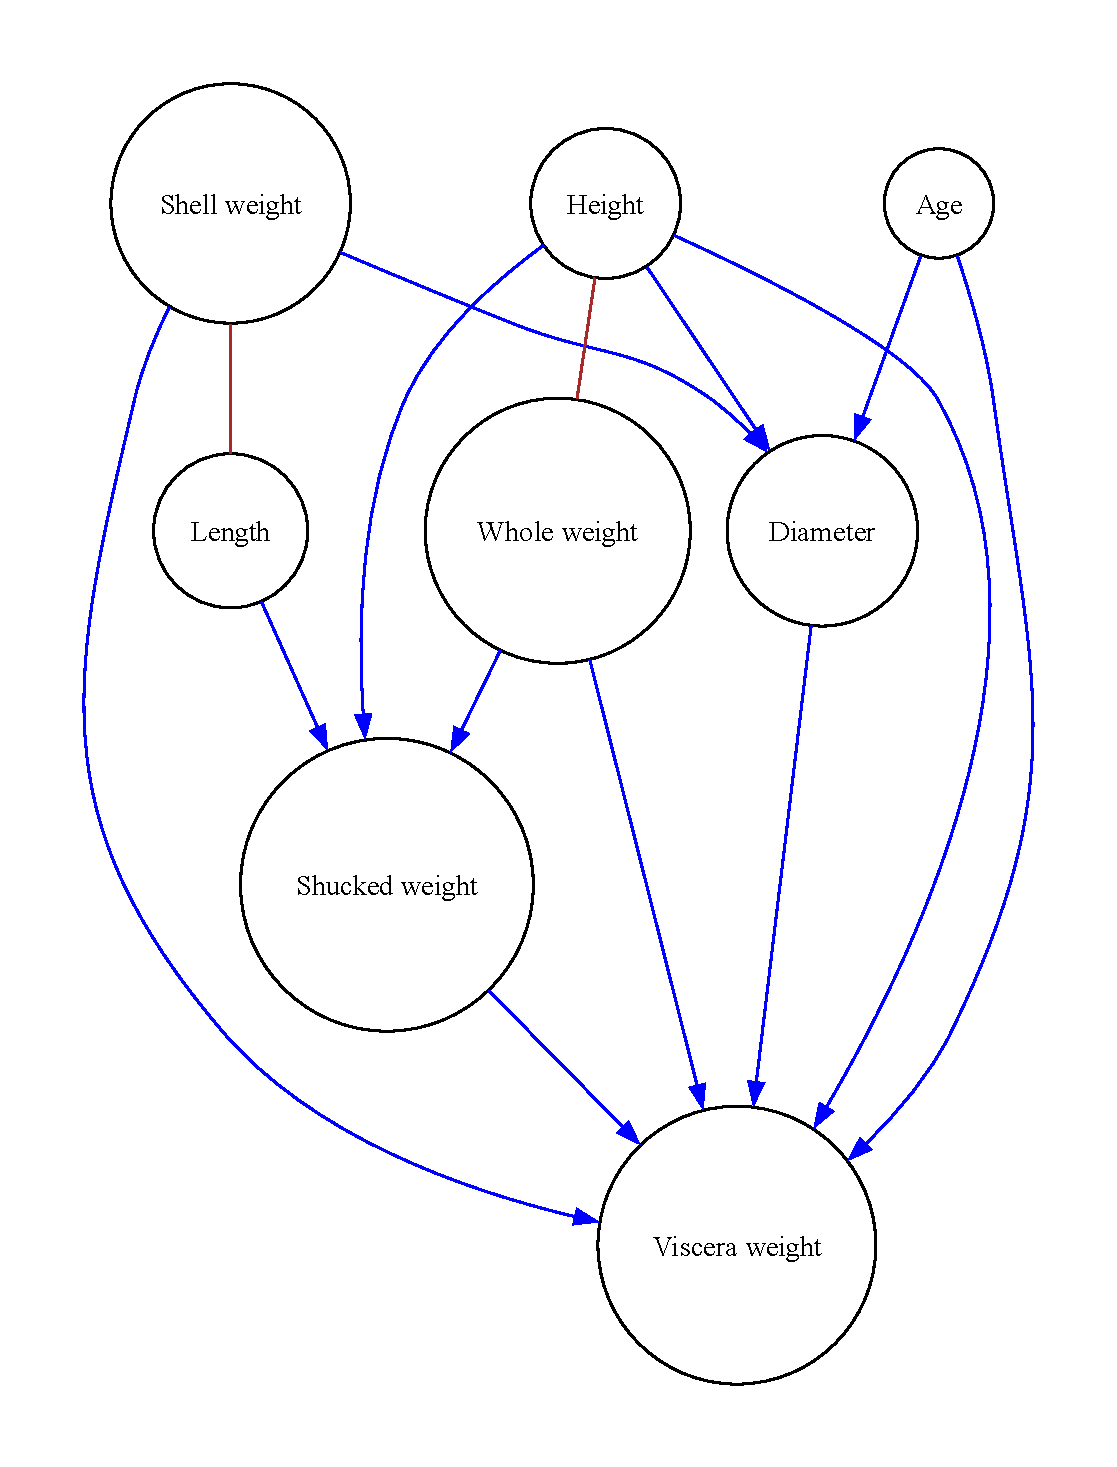
\includegraphics[height=0.3\textheight]{./demo_data/20241104_121546/Abalone/output_graph/initial_graph.pdf}
    \caption{Initial Graph}
\end{figure}

The above is the initial result graph produced by our algorithm.

The analysis reveals a complex web of causal relationships among the variables, indicating that Age influences factors such as Diameter and Viscera weight, suggesting that as organisms age, they tend to have larger diameters and increased viscera weight, which may correlate with overall growth. Length plays a pivotal role as it directly affects both Shell weight and Shucked weight, highlighting the importance of the organism's size in determining these weight metrics. Conversely, Shell weight has a feedback effect on Length and is also linked to Diameter and Viscera weight, implying a bidirectional relationship between these factors. Height emerges as another significant variable, impacting Diameter, Whole weight, Shucked weight, and Viscera weight, indicating that taller organisms are generally heavier and have larger proportions of various anatomical features. Finally, the relationships among Whole weight, Shucked weight, and Viscera weight underscore the interconnectedness of these metrics, suggesting that increases in overall body weight contribute to increases in the weights of the components studied, creating a dynamic interplay between the physical dimensions and the biological attributes of the organisms.

\subsection{Revised Graph}

\begin{minipage}[t]{0.6\linewidth} 
By using the method mentioned in the Section 4.4, we provide a revised graph pruned with Bootstrap and LLM suggestion.
Pruning results are as follows.
        
Bootstrap doesn't force or forbid any edges.
            
The following are force results given by LLM:
            
\begin{itemize}        
\item \textbf{Age $\rightarrow$ Length}: Older abalones tend to be larger in length as age influences growth patterns and size development.
                
\item \textbf{Age $\rightarrow$ Shell weight}: As abalones age, they accumulate more shell mass, leading to an increase in shell weight, which serves as an indicator of growth.
                
\item \textbf{Age $\rightarrow$ Height}: With increasing age, abalones generally exhibit an increase in height, reflecting their overall growth and maturation.
                
\item \textbf{Age $\rightarrow$ Whole weight}: The total weight of an abalone, including its shell and flesh, increases with age due to the overall growth of the organism.
                
\item \textbf{Age $\rightarrow$ Shucked weight}: An increase in age typically results in larger and heavier abalones, which correlates with a higher shucked weight of the meat.
                
\item \textbf{Length $\rightarrow$ Diameter}: As the length of the abalone grows, its diameter also increases, given that these dimensions are related to the overall size of the organism.
                
\item \textbf{Length $\rightarrow$ Height}: The growth in length of abalones is often accompanied by corresponding increases in height, since both are dimensions of the organism's size.
                
\item \textbf{Length $\rightarrow$ Whole weight}: Increased length is associated with an increase in whole weight, as larger abalones generally have more biomass.
                
\item \textbf{Length $\rightarrow$ Viscera weight}: As the length increases, it is likely that the viscera weight will also increase due to the larger overall body size and potential for more internal organs.
                
\item \textbf{Shell weight $\rightarrow$ Height}: The weight of the shell reflects the overall health and condition of the abalone, which can also determine its height as it matures.
                
\item \textbf{Shell weight $\rightarrow$ Whole weight}: There is a strong correlation between shell weight and whole weight, as the shell contributes significantly to the abalone's total mass.
                
\item \textbf{Shell weight $\rightarrow$ Shucked weight}: A heavier shell weight is indicative of a larger abalone, which typically results in a greater amount of meat after shell removal, thereby increasing shucked weight.
                
\item \textbf{Diameter $\rightarrow$ Whole weight}: The diameter measurement is related to the overall size of the abalone and thus is positively correlated with whole weight.
                
\item \textbf{Diameter $\rightarrow$ Shucked weight}: A wider diameter generally means a larger and heavier abalone, which corresponds to a greater shucked weight of the meat.
\end{itemize}
            
The following are directions of remaining undirected edges determined by the LLM:
\begin{itemize}
\item \textbf{Length $\rightarrow$ Shell weight}: As abalones grow, their length tends to increase with age, which in turn leads to an increase in shell weight. This relationship reflects the physical development and structural growth of the abalone, as larger abalones have thicker and heavier shells.

\item \textbf{Height $\rightarrow$ Whole weight}: The height of the abalone is directly related to its overall growth. As the height increases, the overall biomass, reflected in the whole weight, also increases, demonstrating a positive correlation between these two measurements during growth.
\end{itemize}
        
This structured approach ensures a comprehensive and methodical analysis of the causal relationships within the dataset.
        
\vfill
\end{minipage}
\hfill
\begin{minipage}[t]{0.4\linewidth}
    \begin{figure}[H]
        \centering
        \vspace{-0.5cm}
        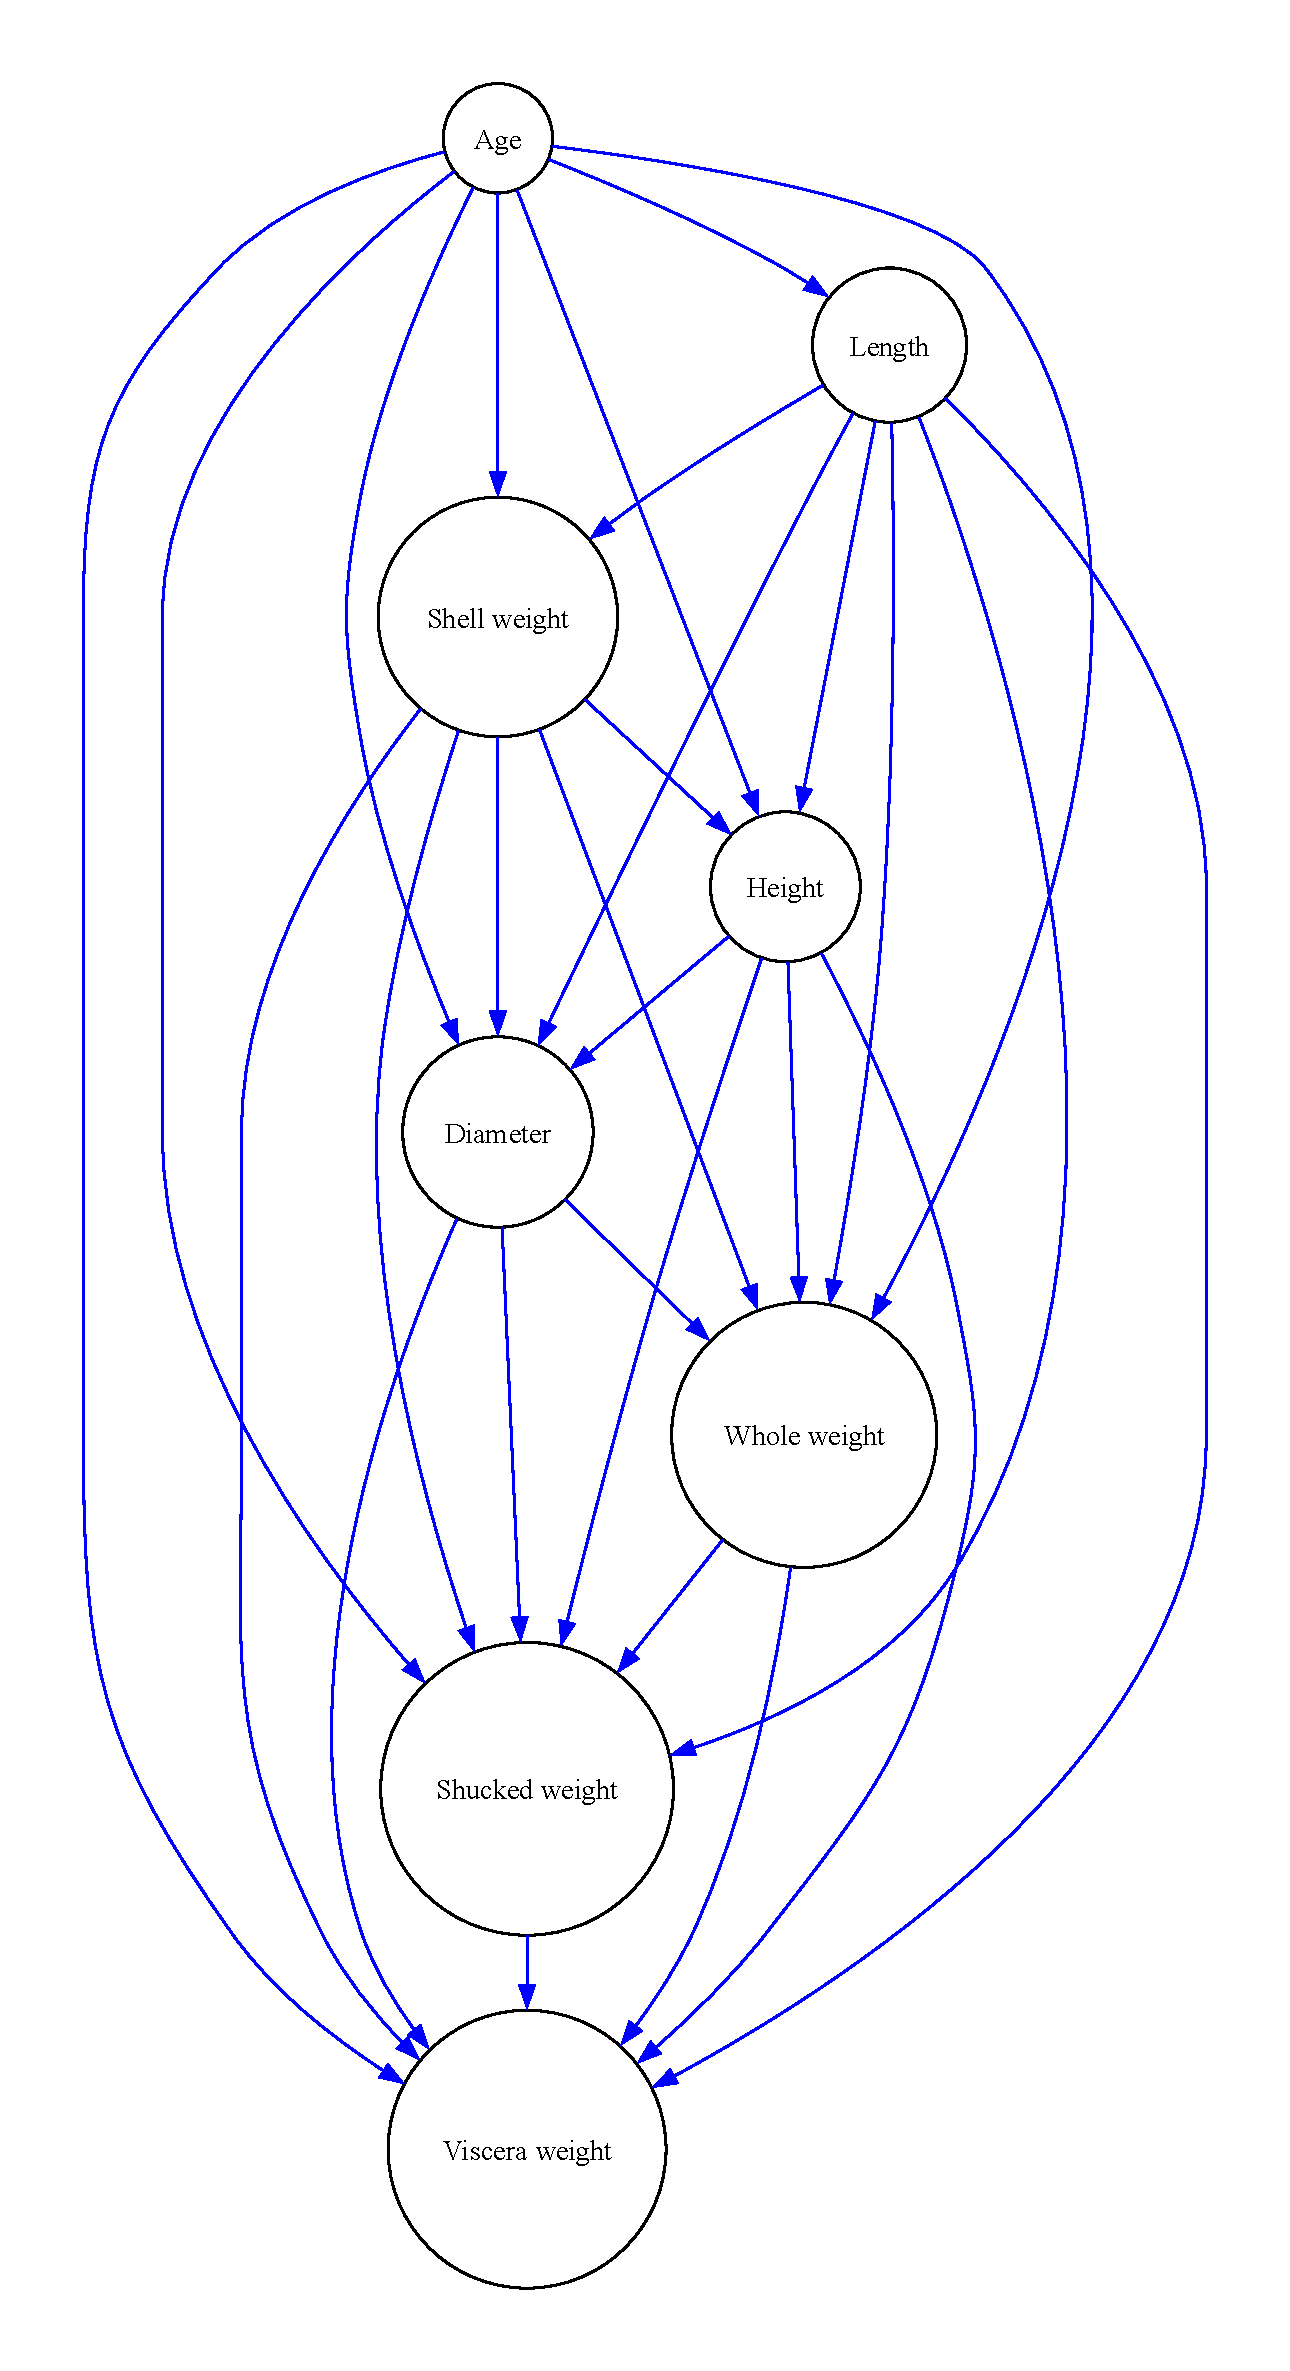
\includegraphics[width=\linewidth]{./demo_data/20241104_121546/Abalone/output_graph/revised_graph.pdf}
        \caption{\label{fig:corr}Revised Graph}
    \end{figure}
\end{minipage}

\subsection{Graph Reliability Analysis}

\begin{figure}[H]
    \centering
    \begin{subfigure}{0.32\textwidth}
        \centering
        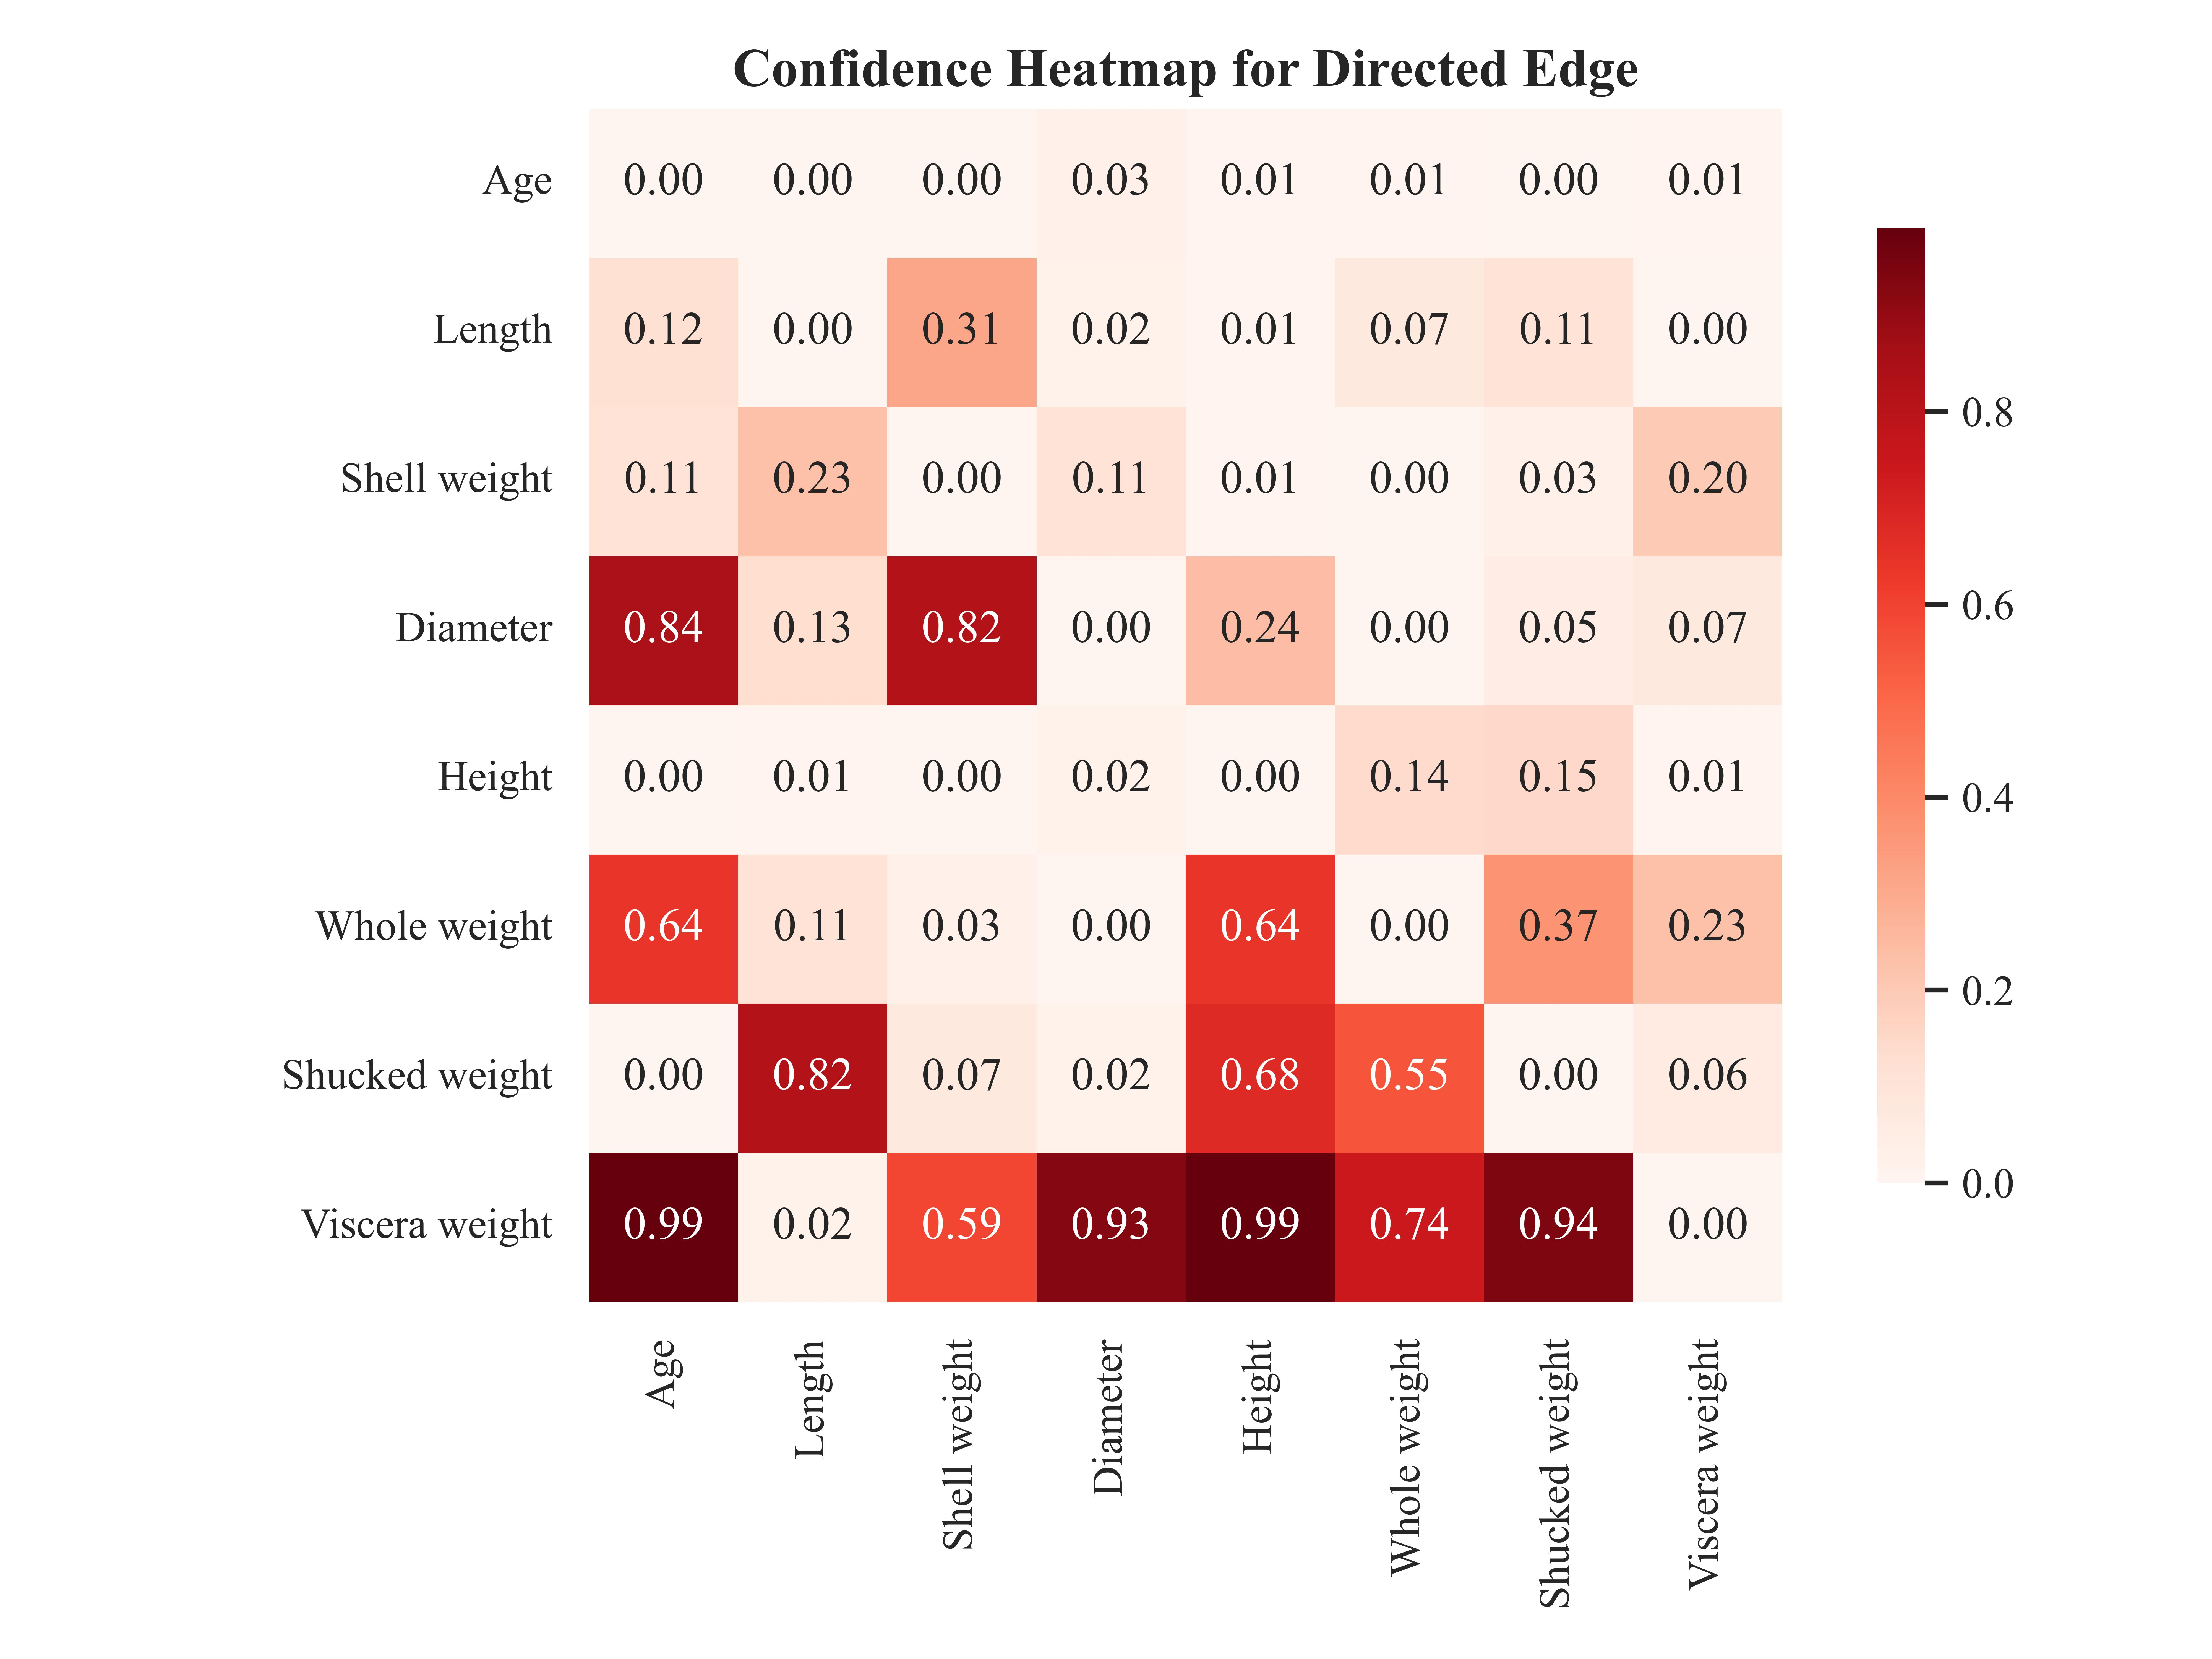
\includegraphics[width=\linewidth]{./demo_data/20241104_121546/Abalone/output_graph/certain_edges_confidence_heatmap.jpg}
        \caption{Directed Edge}
    \end{subfigure}
    \begin{subfigure}{0.32\textwidth}
        \centering
        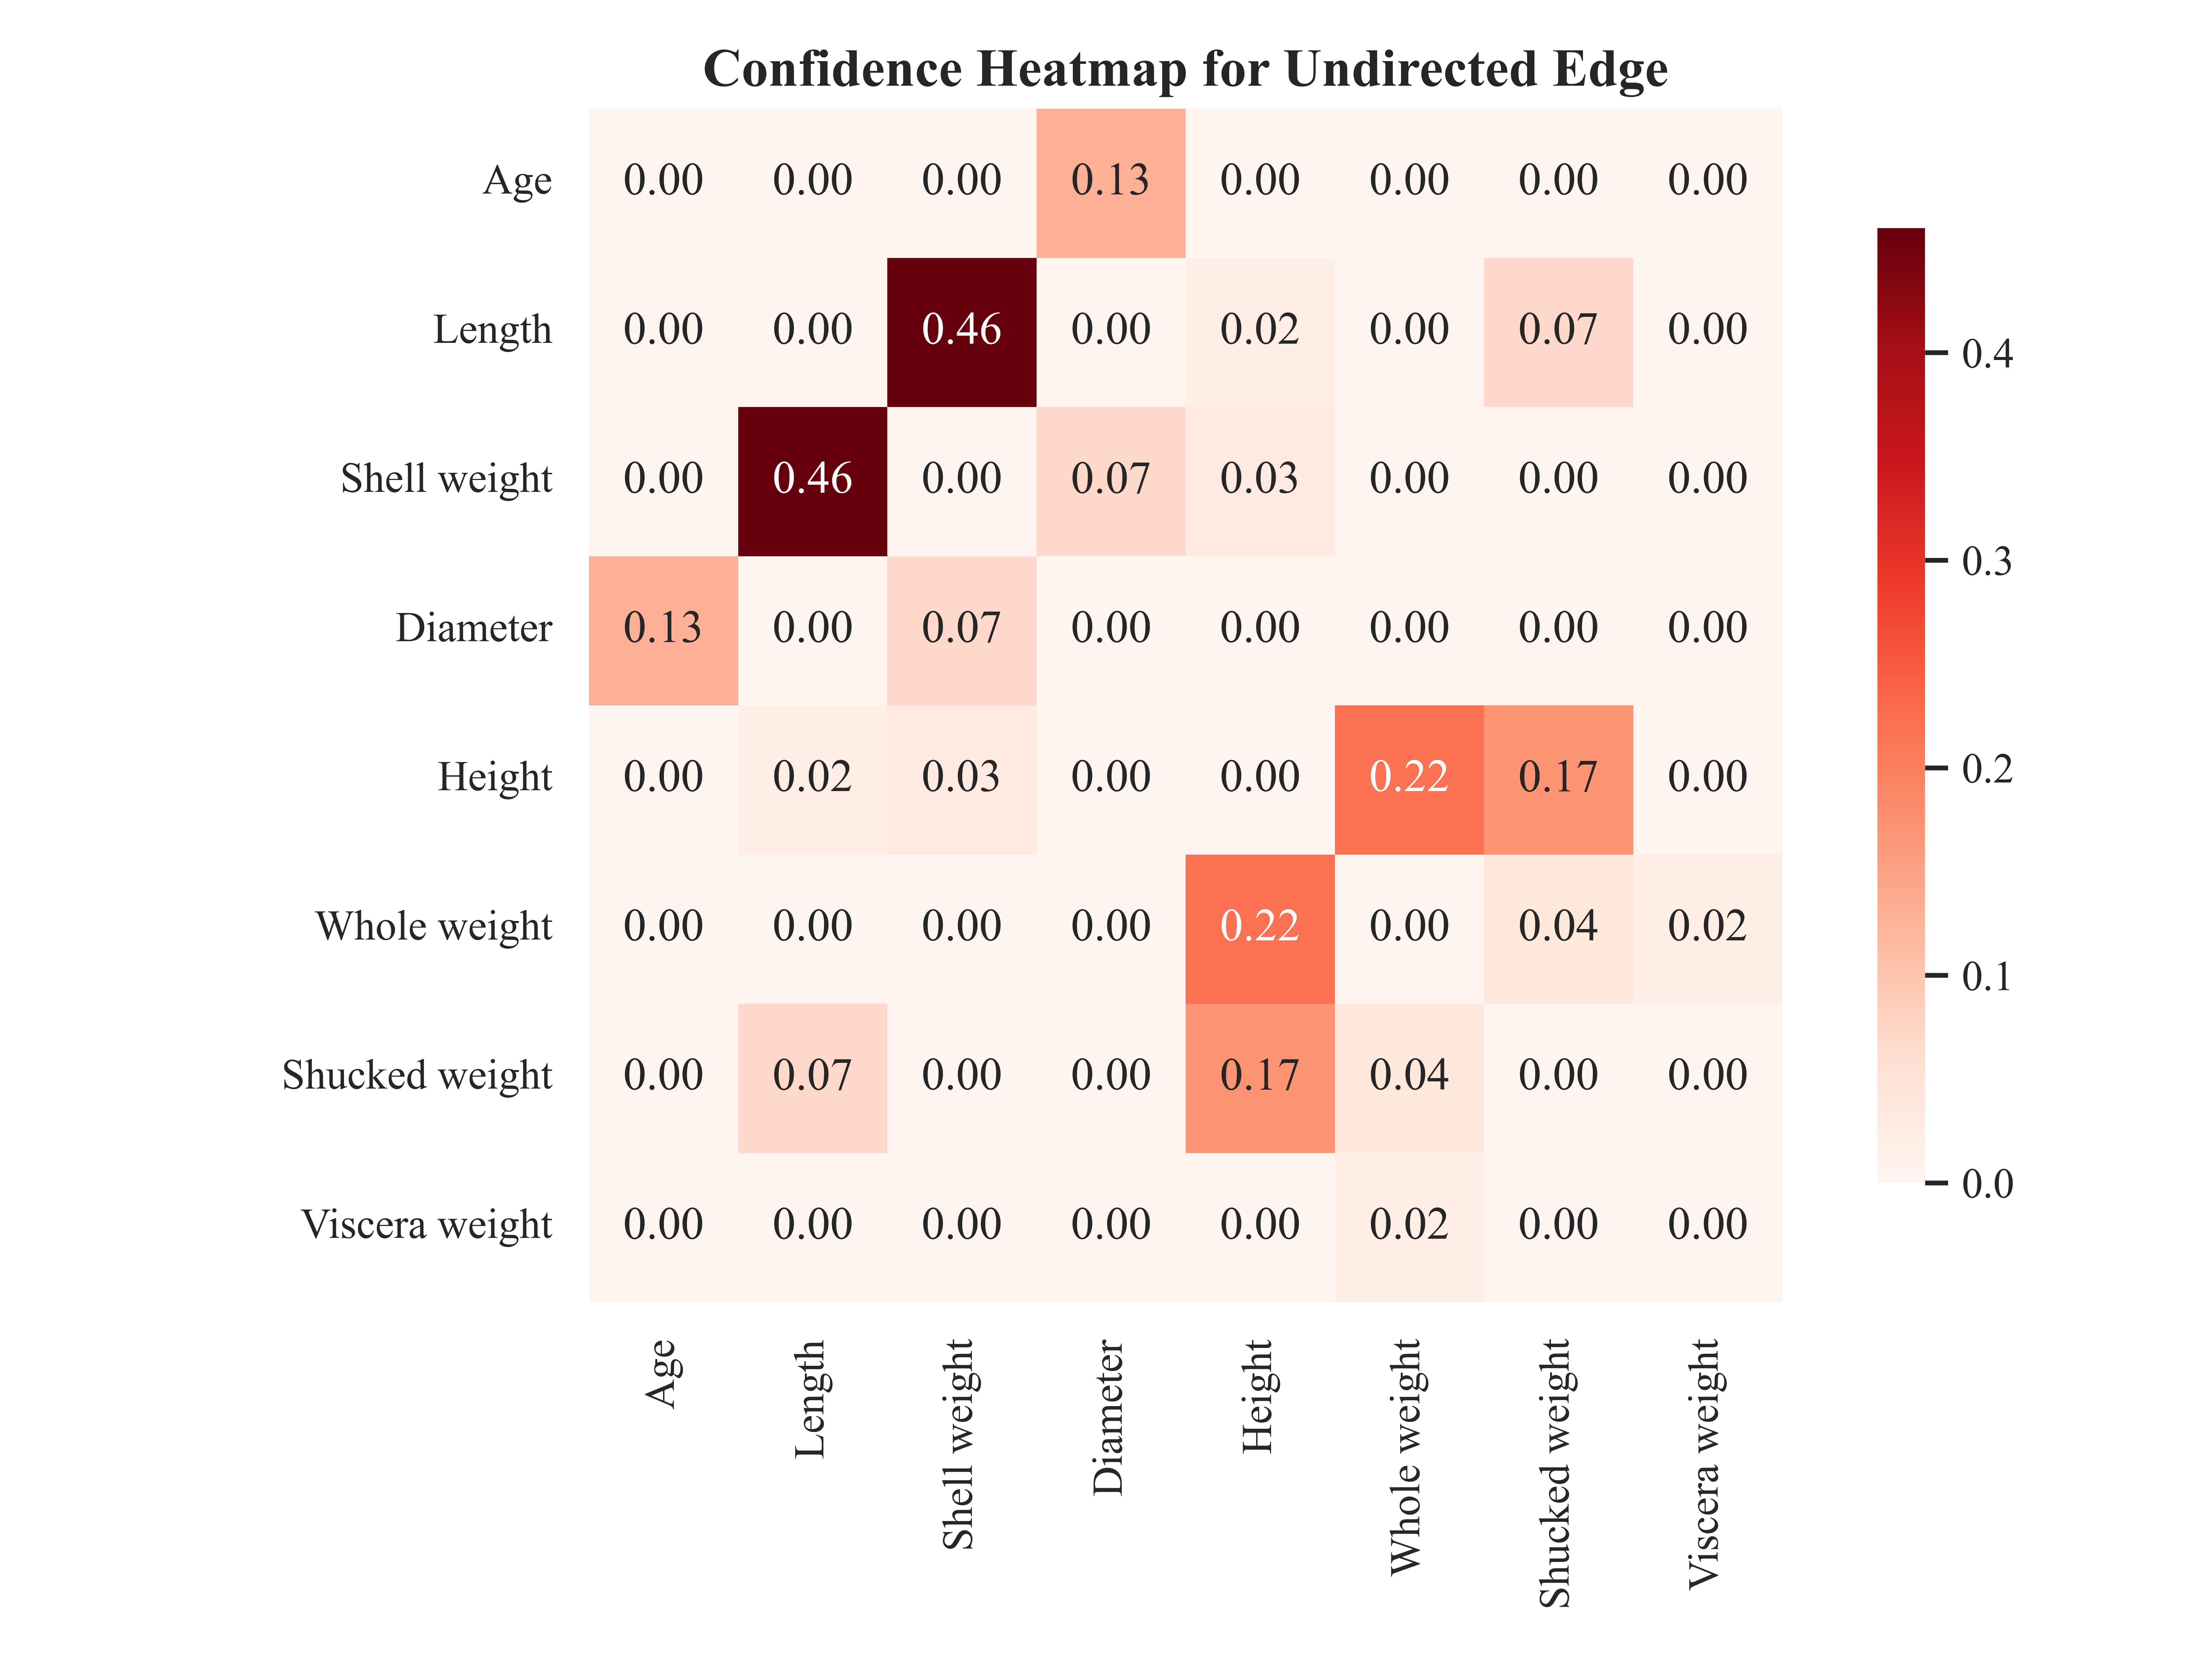
\includegraphics[width=\linewidth]{./demo_data/20241104_121546/Abalone/output_graph/uncertain_edges_confidence_heatmap.jpg}
        \caption{Undirected Edge}
    \end{subfigure}
    \begin{subfigure}{0.32\textwidth}
        \centering
        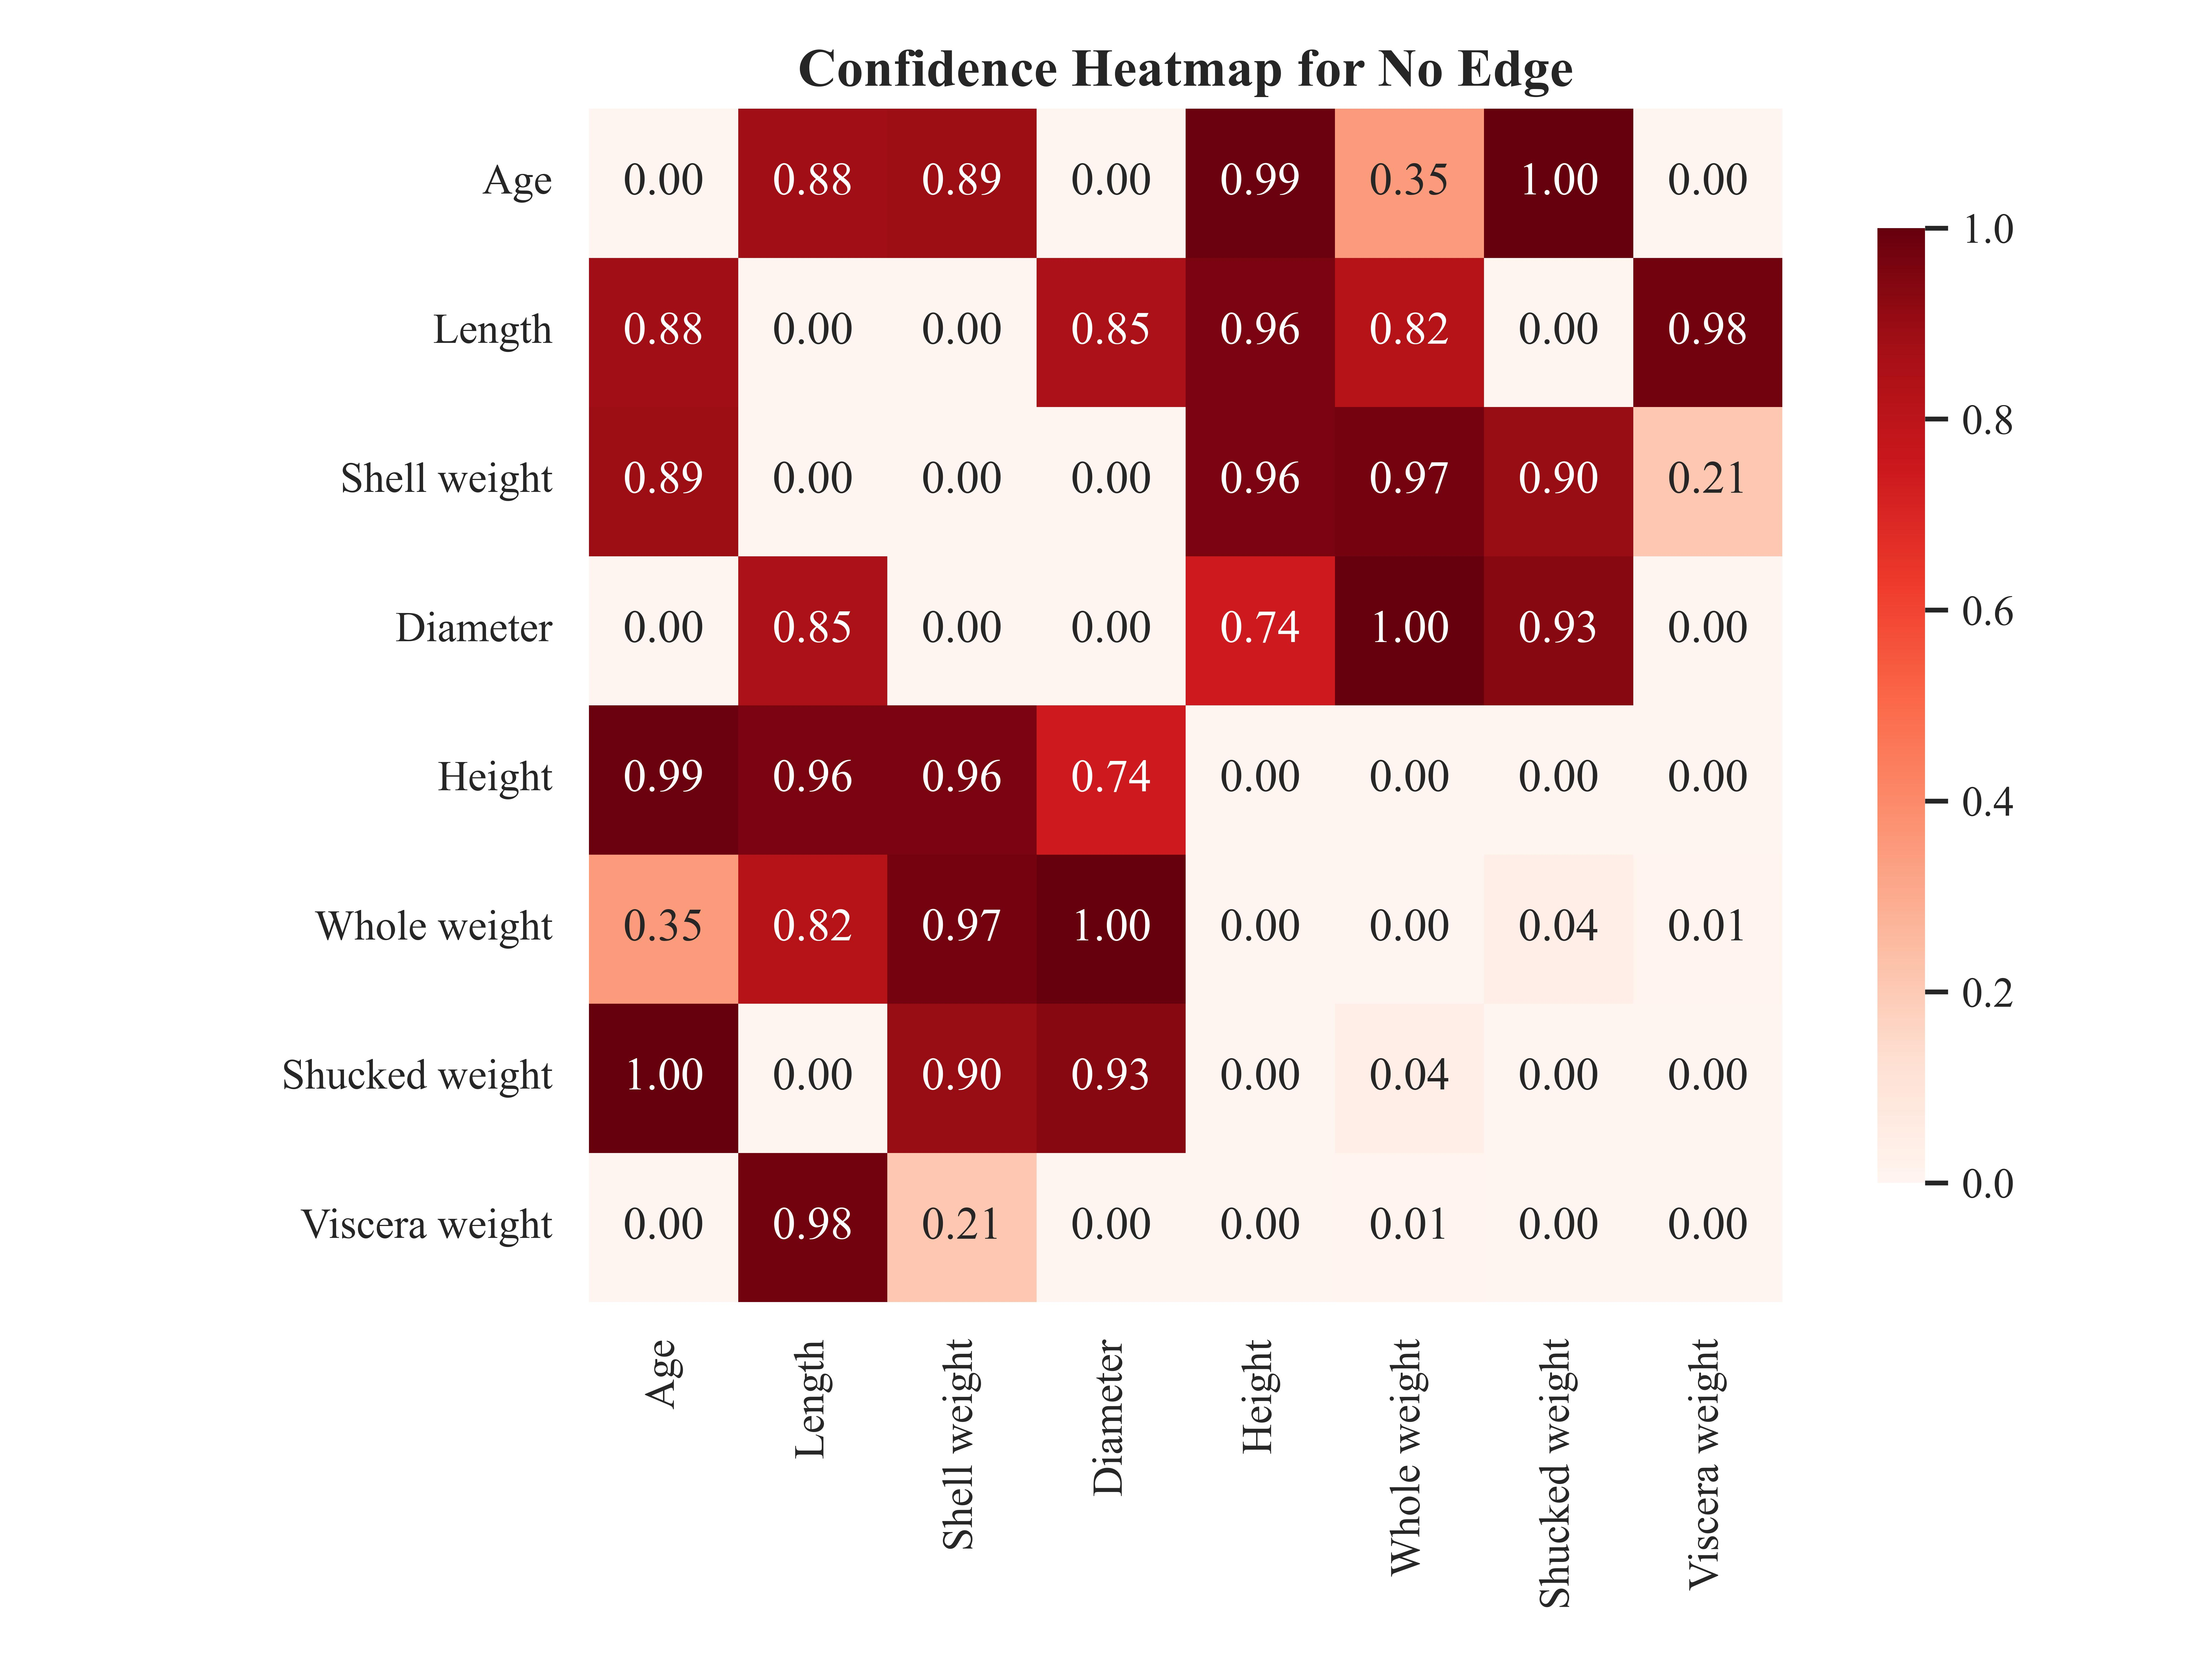
\includegraphics[width=\linewidth]{./demo_data/20241104_121546/Abalone/output_graph/non_existence_confidence_heatmap.jpg}
        \caption{No Edge}
    \end{subfigure}
\caption{Confidence Heatmap of Different Edges}
\end{figure}        
The above heatmaps show the confidence probability we have on different kinds of edges, including directed edge ($\rightarrow$), undirected edge ($-$), No Edge, and probability of no edge. The heatmap of bi-edges is not shown because probabilities of all edges are 0. Based on the confidence probability heatmap and background knowledge, we can analyze the reliability of our graph.

From a statistical perspective, we have high confidence to believe that the edges representing the relationships between Whole weight and its influence on Height (bootstrap probability 0.64), Shucked weight (0.37), and Viscera weight (0.23) exist, indicating strong causal links. Additionally, there is moderate confidence in the edges involving Length impacting Shell weight (0.31) and Shucked weight (0.11), as well as Shell weight influencing Diameter (0.11) and Viscera weight (0.20). Conversely, we have low confidence regarding the edges Age $\rightarrow$ Diameter (0.03) and Age $\rightarrow$ Viscera weight (0.01), indicating that these causal claims are weak. 

However, based on expert knowledge, we know that the growth of abalones fundamentally supports the existence of relationships such as Age influencing Length, Diameter, and Height, as older abalones tend to be larger (these edges, however, are not directly tested in the bootstrap results). Furthermore, it follows that Whole weight will invariably affect both Shucked weight and Viscera weight, given that an increase in total biomass correlates directly with increase in the weight of the meat and viscera. The knowledge about health and reproductive biology also implies relationships between Shucked weight and Viscera weight that were observed in the edges specified.

Therefore, while there is a mix of strong and weak statistical edges in the causal graph, the expert knowledge corroborates several fundamental relationships that support the existence of some edges. However, the low bootstrap probabilities for some relationships also raise concerns about the reliability of the edges suggested by the statistical analysis. Thus, we conclude that the result of this causal graph is moderately reliable, calling for further investigation, especially for edges with low bootstrap probability.
\end{document}